\section{Quantum Search Algorithnms}
Classical search algorithm through $N$ unordered elements $\mathcal{O}(N)$. \\
Quantum Grover's algorithm: $\mathcal{O}(\sqrt{N})$ (given certain predictions).

\subsection{Quantum Oracles}
Search space of $N = 2^n$ elements, labelled $0, 1, ..., N - 1$.
Assume there are $M$ solutions (with $1 \leq M \leq N$). \\
Define corresponding indictor function $f : \{0, ..., N - 1\} \mapsto \{0, 1\}$
by 
\begin{equation}
    f(x) = \begin{cases}
        0, \quad \text{if element $x$ is not a solution} \\
        1, \quad \text{if element $x$ is a solution}
    \end{cases}
\end{equation}

Quantum version of $f$?
$\leadsto$ Quantum "oracle" $U_f$ defined for computational basis states as

\begin{figure}[H]
    \centering
    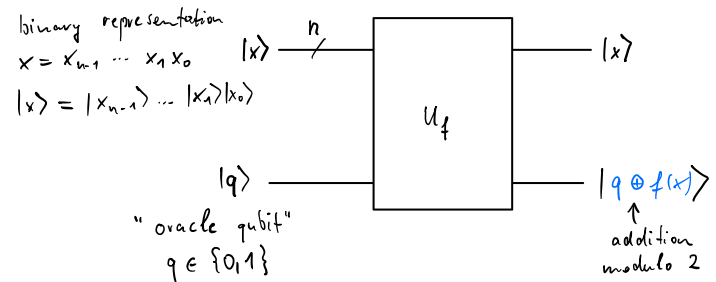
\includegraphics[scale=0.5]{chapters/res/quantum-circuit-oracle.png}
\end{figure}

Note: $U_f$ maps basis states to basis states and satisfies 
\begin{equation}
U_f^2 = I \quad (\text{since } q \oplus f(x) \oplus f(x) = q)
\end{equation}

Thus $U_f$ permutes basis states and is in particular unitary.

Initialize oracle qubit in superposition $\ket{-} = \frac{1}{\sqrt{2}}(\ket{0} - \ket{1})$, 
then 

\begin{equation}
    \ket{x} \otimes \frac{\ket{0} - \ket{1}}{\sqrt{2}}
    \stackrel{U_f}{\mapsto}
    \begin{cases}
        \ket{x} \otimes \frac{\ket{0} - \ket{1}}{\sqrt{2}} & \text{if } f(x) = 0\\
        \ket{x} \otimes \frac{\ket{1} - \ket{0}}{\sqrt{2}} = 
            - \ket{x} \otimes \frac{\ket{0} - \ket{1}}{\sqrt{2}} & \text{if } f(x) = 1
    \end{cases}
\end{equation}

In summary: 
\begin{equation}
    \ket{x} \otimes \frac{\ket{0} - \ket{1}}{\sqrt{2}}
    \stackrel{U_f}{\mapsto}
    \underbrace{{\color{blue}-1^{f(x)}}}_{\text{only this part relevant for the following}}
        \ket{x} \otimes \underbrace{\frac{\ket{0} - \ket{1}}{\sqrt{2}}}_{\text{Oracle qubit unchanged}}
\end{equation}

$\leadsto$ Effective action of oracle

\begin{figure}[H]
    \centering
    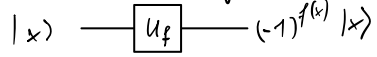
\includegraphics[scale=0.5]{chapters/res/effective-action-oracle.png}
    \caption{Oracle "marks" solution by a phase flip.}
\end{figure}


How could one construct such an oracle without knowing solution already? \\
Example: Factorization of a large integer $m \in \mathbb{N}$:
Finding prime factor of $m$ is "difficult" on a classical computer (no known algorithm with
polynomial runtime in the bit length of $m$). \\
But testing whether a given $x \in \mathbb{N}$ divides $m$ is simple.

Can perform arithmeti operations for trial divisions on a digital quantum computer as well
$\leadsto$ Oracle which recognizes a solution $x$.

\subsection{Grover's Algorithm}
Search space with $N = 2^n$ elements, $M$ solutions. 

\begin{figure}[H]
    \centering
    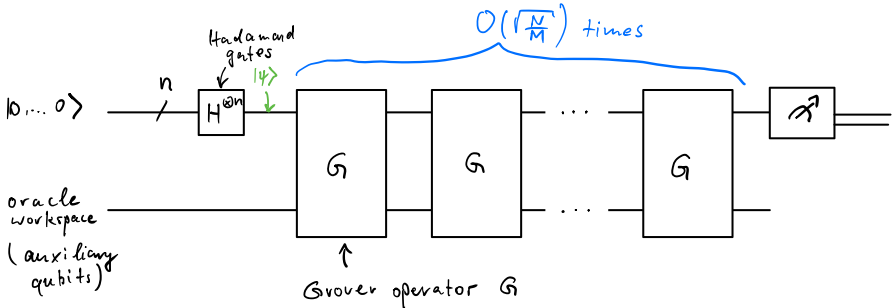
\includegraphics[scale=0.4]{chapters/res/groovers-algorithm.png}
\end{figure}

Initial Hadamard transform: \\

\begin{figure}[H]
    \centering
    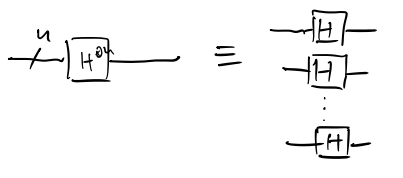
\includegraphics[scale=0.5]{chapters/res/initial-hadamard-transform.png}
\end{figure}
Note: For $x \in \{0, 1\}$:
\begin{equation}
    H \ket{x} = \frac{1}{\sqrt{2}} \sum_{z = 0}^1 (-1)^{z x} \ket{z} 
\end{equation}

Applied to several qubits:

\begin{align}
    H^{\otimes n} \ket{x_1, ..., x_n} 
        &= \underbrace{(H\ket{x_1})}_{\frac{1}{\sqrt{2}} \sum_{z_1 = 0}^1 (-1)^{x_1 z_1} \ket{z_1}}
            \otimes \cdots \otimes (H \ket{x_n}) \\ 
        % 
        &= \frac{1}{\sqrt{2^n}}  \sum_{z = 0}^{2^n - 1} (-1)^{x \cdot z} \underbrace{\ket{z}}_{\text{bit string}}
\end{align}

In particular: 
\begin{equation}
    H^{\otimes n} \ket{0, ..., 0} = \frac{1}{\sqrt{N}} \sum_{z = 0}^{N - 1} \ket{z} =: {\color{green} \statepsi \text{ equal superposition state}}
\end{equation}

Definition of Grover operator G:

\begin{figure}[H]
    \centering
    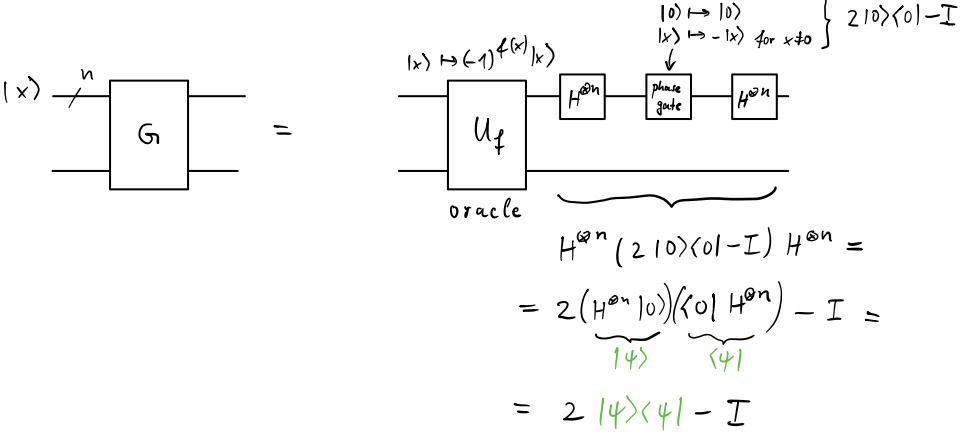
\includegraphics[scale=0.4]{chapters/res/grover-operation-circuit.png}
\end{figure}

In summary 
\begin{equation}
    G := (2 \statepsi \bra{\psi} - I) U_f
\end{equation}


\underline{Geometric interpretation:}

\begin{figure}[H]
    \centering
    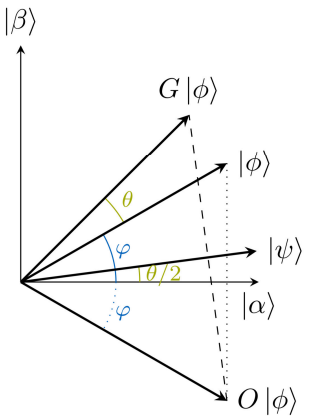
\includegraphics[scale=0.5]{chapters/res/grover-geometric-representation.png}
\end{figure}

Define 
\begin{equation}
    \ket{\alpha} := \frac{1}{\sqrt{N - M}} \sum_{x=0, f(x) = 0}^N \ket{x}
\end{equation}

\begin{equation}
    \ket{\beta} := \frac{1}{\sqrt{M}} \sum_{x=0, f(x) = 1}^N \ket{x}
\end{equation}


Angle $\vartheta$ defined by $\sin \frac{\vartheta}{2} = \sqrt{\frac{N}{M}}$
such that $\statepsi = \cos \frac{\vartheta}{2} \ket{\alpha} + \sin \frac{\vartheta}{2} \ket{\beta}$


Note: By definition $U_f \ket{a} = \alpha$, $U_f \ket{\beta} = -\ket{\beta}$ 
$\leadsto U_f$ is a reflection about $\ket{\alpha}$ within subspace spanned by $\ket{\alpha}$ and $\ket{\beta}$ \\

Likewise $2 \statepsi \bra{\psi} - I$ is a reflection about $\statepsi$:

\begin{figure}[H]
    \centering
    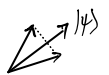
\includegraphics[scale=0.5]{chapters/res/psi-reflection-diagram.png}
\end{figure}

Since $\statepsi$ is part of subspace spanned by $\ket{\alpha}$ and $\ket{\beta}$, 
$G$ leaves subspace invariant! \\
Thus $G$ is a product of two reflections $\leadsto G$ is a rotation by angle 
$\vartheta$
\begin{align}
    \ket{\phi} &= \cos{\varphi} \ket{\alpha} + \cos{\varphi} \ket{\beta} \\
    \leadsto G \ket{\phi} &= \cos{(\varphi + \vartheta)} \ket{\alpha} + \cos{(\varphi + \vartheta)} \ket{\beta}
\end{align}


For $k$ applicants of $G$:
\begin{equation}
    G^k \ket{\phi} = \cos{(\phi + k \cdot \vartheta)} \ket{\alpha} 
        + \sin{(\phi + k \cdot \vartheta)} \ket{\beta}
\end{equation}

For initial state $\statepsi$: $\psi = \frac{\vartheta}{2}$
\begin{equation}
    G^k \ket{\phi} = \cos{((k + \frac{1}{2}) \vartheta)} \ket{\alpha} 
        + \sin{((k + \frac{1}{2}) \vartheta)} \ket{\beta}
\end{equation}

Goal: Rotate to $\ket{\beta}$, i.e. $(k + \frac{1}{2}) \vartheta \stackrel{!}{=} \frac{\pi}{2}$

since $\sin{\frac{\vartheta}{2}} = \sqrt{\frac{M}{N}}$ for $M \ll N \quad \vartheta \approx 2 \sqrt{\frac{M}{N}}$

Thus need $\mathcal{O}(\sqrt{\frac{M}{N}})$ rotations 
($k \cdot \vartheta$ should be $\mathcal{O}(1), k \approx \frac{1}{\vartheta}$).

Final step: standard measurement will collapse quantum state (with high probability)
to a basis state forming $\ket{\beta}$, i.e. a solution!


\subsection{Optimality of the search algorithm}

Goal: Show that any quantum search algorithm needs $\Omega(\sqrt{N})$ oracle calls
$\leadsto \mathcal{O}(\sqrt{N})$ is already optimal.

For simplicity: Single solution $x$
Recall that oracle flips sign of solutions:
$O_x = I - 2 \ket{x}\bra{x} \quad $ (denoted $U_f$ in previous section) \\
Most general form of algorithm: Oracle calls interleaved with unitary $U_1, U_2, ...$ \\

State after $k$ steps:
\begin{equation}
    \ket{\psi_k^\star} = U_k O_x U_{k-1} O_x \cdots U_1 O_x \ket{\psi_0}
\end{equation}

We also define

\begin{equation}
    \ket{\psi_k} = U_k U_{k-1} \cdots U_1 \ket{\psi_0}
\end{equation}

Strategy of proof: Upper bound of 
\begin{equation}
    D_k := \sum_{x = 0}^{N - 1} || \underbrace{\ket{\psi_k^\star}}_{\text{Case that $x$ is a solution}} 
    - \ket{\psi_k} ||^2
\end{equation}

$D_k$ grows as $\mathcal{O}(k^2)$, but must be $\Omega(N)$ to distinguish between $N$ alternatives.


First show that $D_k \leq 4 k^2$ by induction:

$k = 0 \leadsto D_0= 0$ {\color{green} $\checkmark$}

$k \mapsto k + 1$:

\begin{align*}
    D_{k + 1} &= \sum_x || O_x \ket{\psi_k^\star} - \ket{\psi_k} ||^2 \\
    &= \dots
\end{align*}

Rest of proof in the official script on Moodle.

In summary: $\underbrace{D_k \leq 4 \cdot k^2 \quad \text{and} \quad D_k \geq c \cdot N}
    _{k \geq \sqrt{\frac{cN}{4}} \leadsto \text{Number of oracle evaluations}}$


Thought experiment: If it was possible to search using $\mathcal{O}(log(n))$ oracle
calls, then a QC could solve NP-complete problems efficiently: 
Just search through $2^w(n)$ witnesses using $w(n)$ oracle calls where $w(n)$ is 
the bit length of a witness.